\documentclass[12pt, letterpaper, titlepage]{article}

\usepackage{graphicx}
\usepackage{hyperref}

\author{Saba Saba}
\title{\textbf{TSK Typer} \\
\hrulefill \\
Finger Positioning Rules}

\begin{document}
\maketitle

\tableofcontents
\newpage
\listoffigures
\newpage

\section{Finger Positions}
\subsection{General Rules}
\begin{figure}[h]
\centering
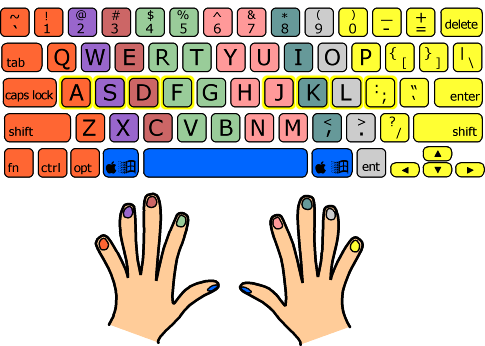
\includegraphics[width=0.5\textwidth]{which_fingers.png}
\caption{Finger-to-key mapping~\cite{hudson.misc}}
\label{Mapping}
\end{figure}
When the typist is not typing, each finger must rest on the home row.
Due to the structure of the hand, the finger-to-key mapping described in figure~\ref{Mapping} is used.
This mapping illustrates how each finger generally moves in a vertical fashion along the keyboard.
The main exceptions are the pinkies, the index fingers and the thumbs:
pinkies are used to reach keys on the outer ends of the keyboard, the index fingers are used for the middle of the keyboard and the thumbs focus on the bottom of the keyboard~\cite{hudson.misc}.

Some other rules to follow are:
\begin{itemize}
\item The fingers must remain as close to the home row as possible, and should exhibit minimal movement~\cite{rapid.misc}.
\item The \textbf{Shift} key must always be pressed with the hand opposite the current typing hand~\cite{rapid.misc}
\end{itemize}

\subsection{Simplified Typing}
\label{simplified}
Assume that a typist begins in the resting position.
The typist presses a single key before returning to the resting position.
This results in a simple validation algorithm for determining correct positioning:
\begin{enumerate}
\item Map the pressed key to a finger according to figure~\ref{Mapping}
\item Ensure that each finger not equal to the above finger is resting on a home row key
\end{enumerate}

\subsection{Fast Typing}
Since the fingers should be as close to the home row as possible,
it is reasonable to assume that a typist will typically exhibit the simplified typing characteristics exhibited in section~\ref{simplified}.
However, a fast typist will anticipate future characters.
Additionally, the typist may still have fingers in midair due to typing preceding characters.
Hence, the algorithm described in section~\ref{simplified} can be updated to the following:
\begin{enumerate}
\item Map the pressed key to a finger according to figure~\ref{Mapping}
\item Ensure that each finger not equal to the above finger is resting on a home row key
\item For each home row key not touched by a finger, determine if the corresponding finger is mapped to a character directly preceding or succeeding the current character
\end{enumerate}

\bibliographystyle{ieeetr}
\clearpage
\phantomsection
\addcontentsline{toc}{section}{\textbf{References}}
\bibliography{report}
\end{document}
